\documentclass[11pt]{article}
\usepackage{graphicx}    % needed for including graphics e.g. EPS, PS
\topmargin -1.5cm        % read Lamport p.163
\oddsidemargin -0.04cm   % read Lamport p.163
\evensidemargin -0.04cm  % same as oddsidemargin but for left-hand pages
\textwidth 16.59cm
\textheight 21.94cm 
%\pagestyle{empty}       % Uncomment if don't want page numbers
\parskip 7.2pt           % sets spacing between paragraphs
%\renewcommand{\baselinestretch}{1.5} % Uncomment for 1.5 spacing between lines
\usepackage{amsmath}
\usepackage{amsfonts}
\usepackage{amsthm}
\usepackage{verbatim}
\usepackage{subfigure}
\parindent 0pt		 % sets leading space for paragraphs
\author{by Erik Waingarten and Fermi Ma}
\title{Data Structures Final Project:\\
A Linear Programming Approach to Dynamic Optimality}

\newtheorem{theorem}{Theorem}
\newtheorem{lemma}[theorem]{Lemma}
\begin{document}         
\maketitle

\section{Introduction}

We consider the the points in the plane problem. The problem is defined as follows:

\vbox{
\noindent
\begin{quote}
Given a set $P$ of $n$ points $(x_i,y_i)$ in the $xy$ plane, no two on a common row or column, find the minimal point set $Q \supseteq P$ such that for any two points in $Q$ not on a common row or column, the rectangle they span contains another point in $Q$.
\end{quote}
}

Point sets $Q$ that satisfy the condition that any two points in $Q$ that span a rectangle contain another point in $Q$ are commonly referred to as \emph{arborally satisfied} point sets.

Note that the problem has $|Q| = \Omega(n)$ since $P \subset Q$. Furthermore, $|Q| = O(n^2)$ trivially since we could fill in every intersecting point (see Figure~\ref{fig:instance}). However, there is another bound which sets $|Q| = O(n\log n)$. The solution was communicated verbally to us by Erik Demaine. Let $m$ be the median in the $x$ axis of $P$, this divides $P$ into two sets of size $O(\frac{n}{2})$. Now for each $(x,y) \in P$, let $(m, y) \in Q$. Then recursively solve both subsets of size $O(\frac{n}{2})$. Note that for every two points, they will be divided by the recursion at some point. This means that there is a point in rectangle. This gives the recursion $|Q| = T(n) = 2T(\frac{n}{2}) + O(n)$, therefore, $|Q| = O(n \log n)$. 

The same bounds arise from knowing that each arborally satisfied set corresponds to an access sequence of a binary search tree algorithm. CITE HERE.

We show an integer linear program whose optimum gives an $O(1)$ approximation problem. It is natural to consider the grid of intersection points ``induced" by the set of points $P$: extend horizontal and vertical lines through each point in $P$ and restrict attention to the $O(n^2)$ intersections of these lines. This is because any points off the grid can be moved to points that are grid intersections. Figure~\ref{fig:instance} shows an example of how a instance of the problem might look like.

\begin{figure}
\centering
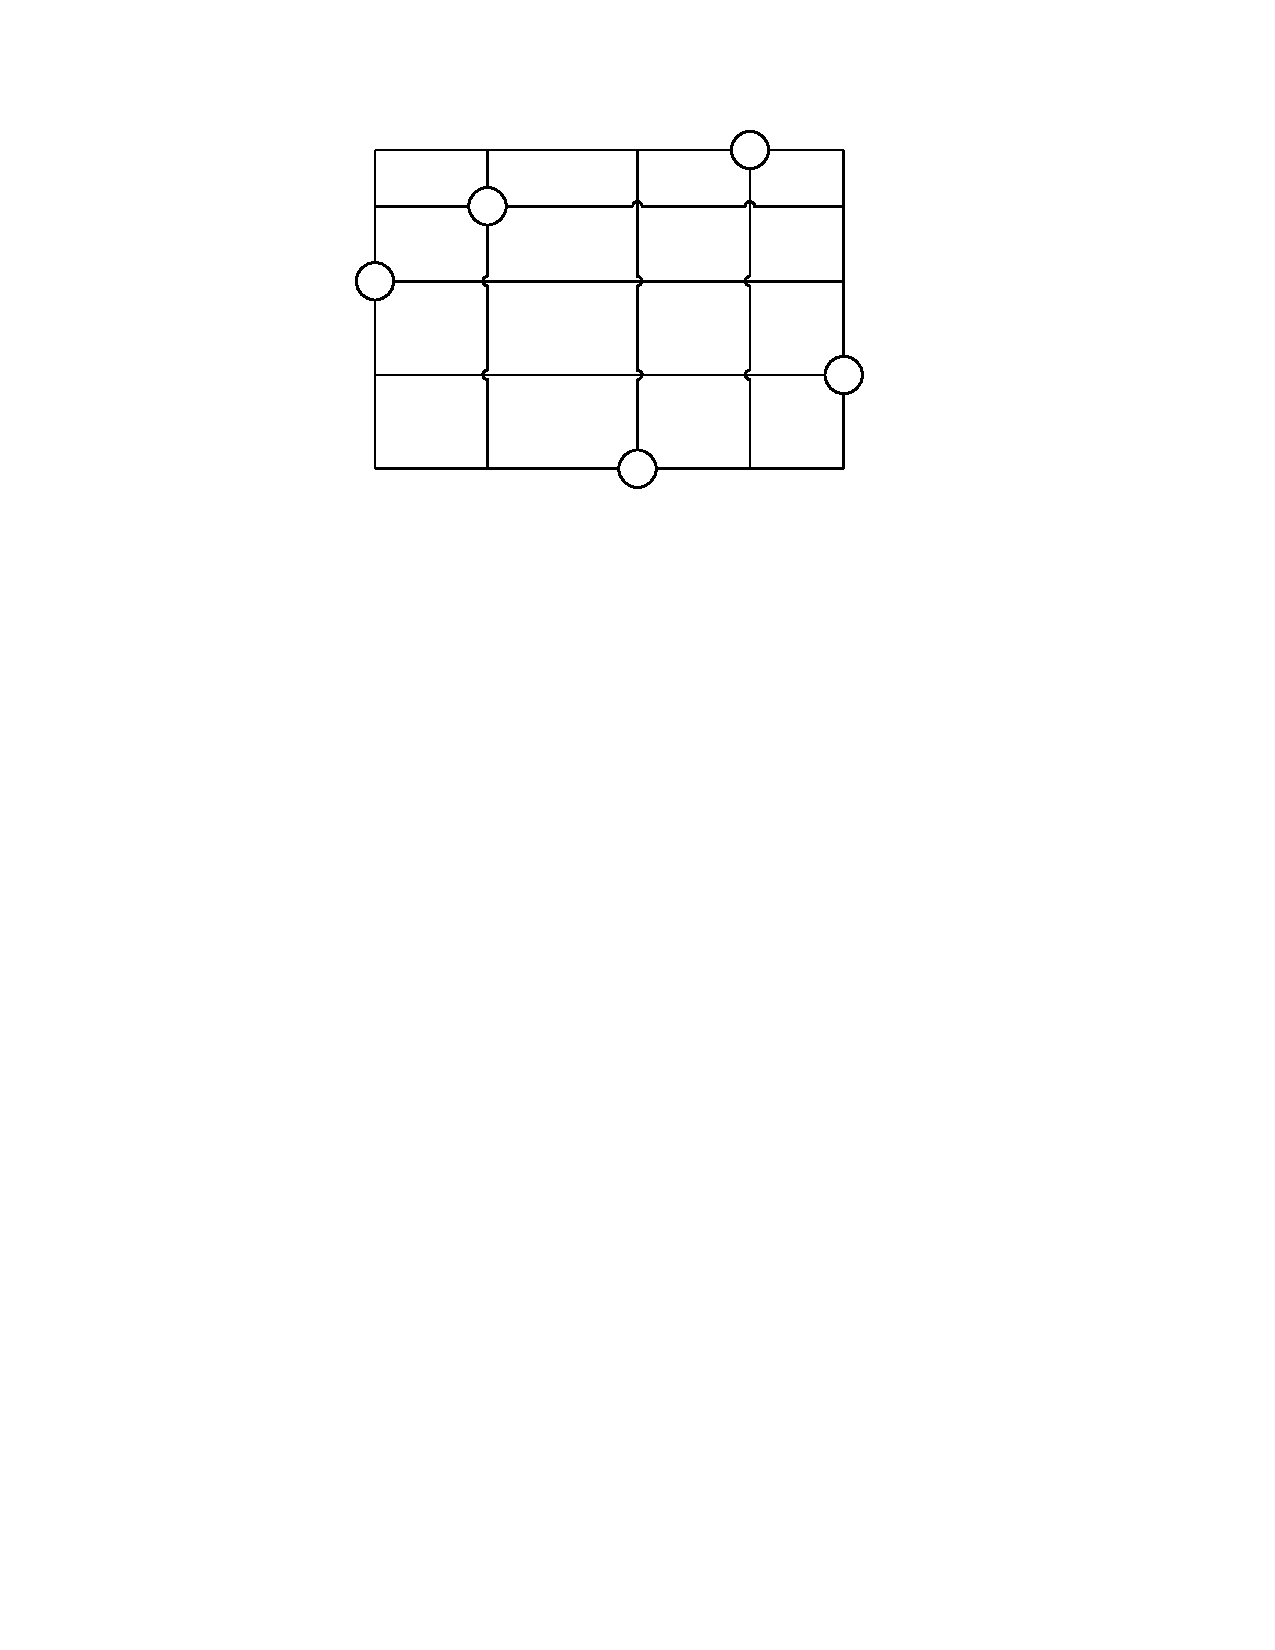
\includegraphics[width=0.3\linewidth]{instance.pdf}
\caption{Instance of points in the plane}
\label{fig:instance}
\end{figure}

We can assign an indicator variable to each grid point, where the variable is set to 1 if the point is included and is 0 otherwise. This gives the obvious objective of minimizing the sum of all variables. In this paper, we restrict our attention to linear programs that follow this model. While other linear programming approaches almost certainly exist, this sort of setup certainly feels the most natural.

\section{A First Attempt}

We set up the indicator variables as explained in the introduction, labeling them as $b_{jk}$, where $j$ and $k$ are labels on the grid intersection points (labelled so that $b_{00}$ is the lower left grid point, $b_{01}$ is the point directly above, and $b_{10}$ is the point directly to the right).

Consider the following set of constraints:

\begin{align}
2b_{ij} + 2b_{nm} - \left(\sum_{i \leq k \leq n}\sum_{j\leq l \leq m} b_{kl}\right) &\leq 1  \hspace{.3in} \forall i<n, j<m \\
2b_{im} + 2b_{nj} - \left(\sum_{i \leq k \leq n}\sum_{j\leq l \leq m} b_{kl}\right)  &\leq 1  \hspace{.3in} \forall i<n, m<j
\end{align}

We claim that these constraints exactly capture arboral satisfaction. Constraints of type (1) correspond to all possible ``positive" rectangles, and constraints of type (2) correspond to all possible ``negative" rectangles.

If we look at constraints of type (1), the vertices corresponding to variables $b_{in}$ and $b_{jm}$ are present, those variables are set to 1 and sum to 4, and this forces the following term in parenthesis to be at least 3 in order for the constraint to be satisfied, however, we know that $b_{in}$ and $b_{jm}$ are inside the parenthesized term, so we need to find one more additional point in the parenthesized term that is set to $1$. The term in parenthesis corresponds to all points in the rectangle spanned by these vertices, and so forcing one of those variables to be 1 is equivalent to ensuring that the rectangle is satisfied. The constraints of type (2) work the same way.

An easy way to think of the constraints is that we are taking the sum of the points that create a rectangle minus every point inside that rectangle which is not the set points, and that this must be less than 1. This says that if both points of the corners are set to 1, then the sum will be 2, which means that there must be at least one point inside the rectangle set to 1. Thus the rectangle is satisfied. 

If the two corner vertices are not present, the positive terms in the constraint are at most 1, and so the constraint is satisfied no matter what the term in parenthesis is.

If we have such constraint for every possible rectangle, we will have an arborally satisfied set. Note that this integer linear program will solve for exactly the optimal solution.

The primary issue with writing constraints like this is that they are possibly quadratic in size, so they are harder to work with. We can simplify the constraints to be linear in size and only sacrifice a constant factor to the optimum. Since we are focused on solving dynamic optimality, giving up a constant factor is fine.

\section{A Second Attempt: Reducing Constraint Size}

To set up linearly sized constraints, we need a simple lemma.

\begin{lemma}
Any arborally satisfied point set can be modified with $O(1)$ multiplicative overhead so that all the rectangles are satisfied by grid points that lie on their edges.
\end{lemma}

\begin{proof} We consider the process of adding points to satisfy unsatisfied rectangles. Consider any unsatisfied negative rectangle, with vertices $v_1 = (0,0)$ and $v_2 = (a,b)$. Suppose it is optimal to satisfy this rectangle by filling in a point not in the rectangle's edge, at vertex $v_3 = (c,d)$ where $c < a$ and $d< b$.

We claim that instead of placing vertex $v_3$, we could have placed the two vertices $(c,b)$ and $(a,d)$. These two vertices clearly satisfy the original rectangle defined by $v_1$ and $v_2$, so the only worry now is that $v_3$ was placed ``optimally" to satisfy other rectangles that intersect this rectangle (and are defined by vertices that lie entirely outside this rectangle). But we note that these two new vertices $(c,b)$ and $(a,d)$ will satisfy any such rectangle that $v_3 = (c,d)$ might have satisfied. Thus, we can simply replace this vertex with these two vertices, and lose at most a factor of 2.

Note that a symmetric argument works for any given positive rectangle

\end{proof}

We claim that the following set of constraints captures arboral satisfaction: 

\begin{align}
b_{ij} + b_{nm} - \left(\sum_{l=i+1}^{n-1} (b_{lj}+b_{lm}) + \sum_{l=j+1}^{m-1} (b_{il} + b_{nl}) + b_{im} + b_{nj} \right) &\leq& 1 & \hspace{.3in} \forall i<n, j<m \\
b_{im} + b_{nj} - \left(\sum_{l=i+1}^{n-1} (b_{lj}+b_{lm}) + \sum_{l=j+1}^{m-1} (b_{il} + b_{nl}) + b_{ij} + b_{nm} \right) &\leq& 1 & \hspace{.3in} \forall i<n, j<m
\end{align}

Constraints of type (3) correspond to all possible ``positive" rectangles, and constraints of type (4) correspond to all possible ``negative" rectangles. This captures arboral satisfaction for the same reason that the constraints of types (1) and (2) do. The only difference is that these constraints only look at vertices on the edges of rectangles. Figure~\ref{fig:rectangles} gives the graphical interpretation of the contraints, where he white circles are added  and the black circles are subtracted, the black lines correspond to all the points in between being subtracted.

\begin{figure}
\centering
\subfigure[Positive rectangle]{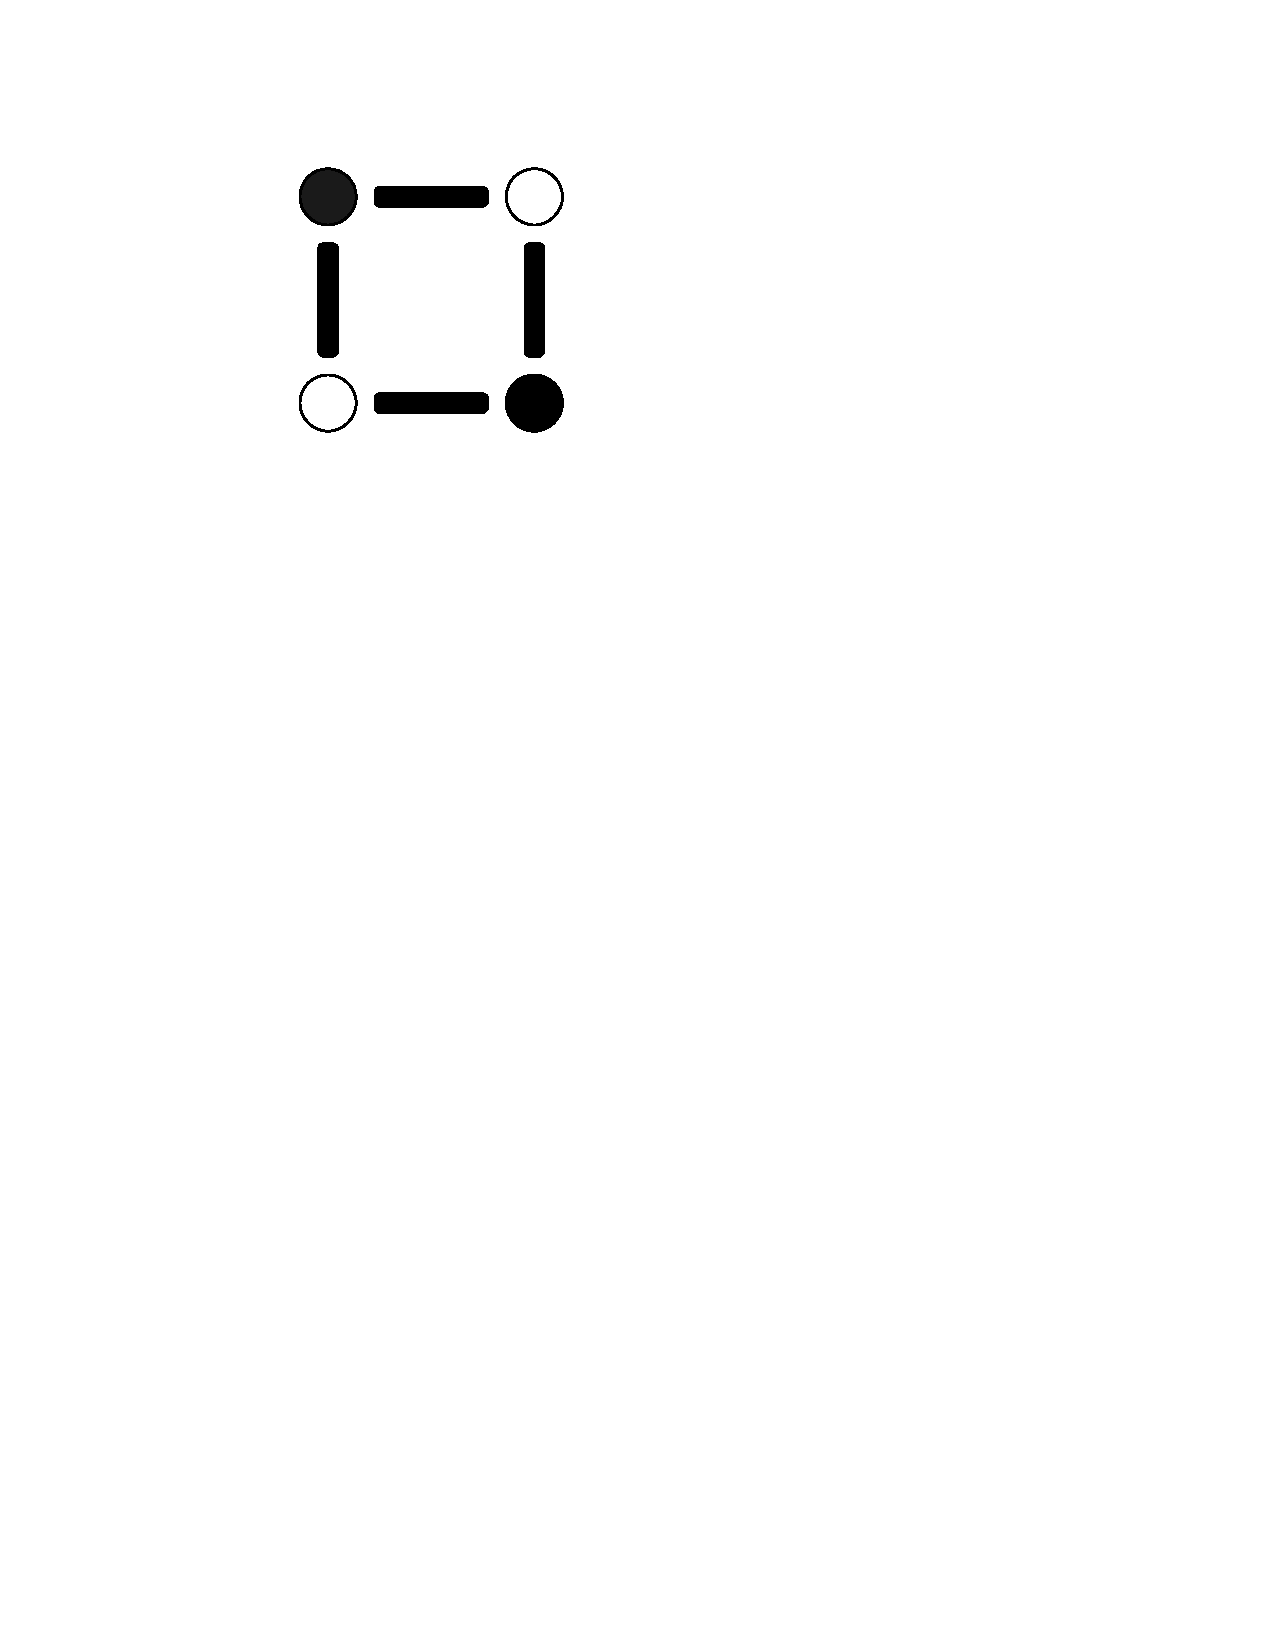
\includegraphics[width=0.2\linewidth]{positive.pdf}\label{fig:positive}}
\subfigure[Negative rectangle]{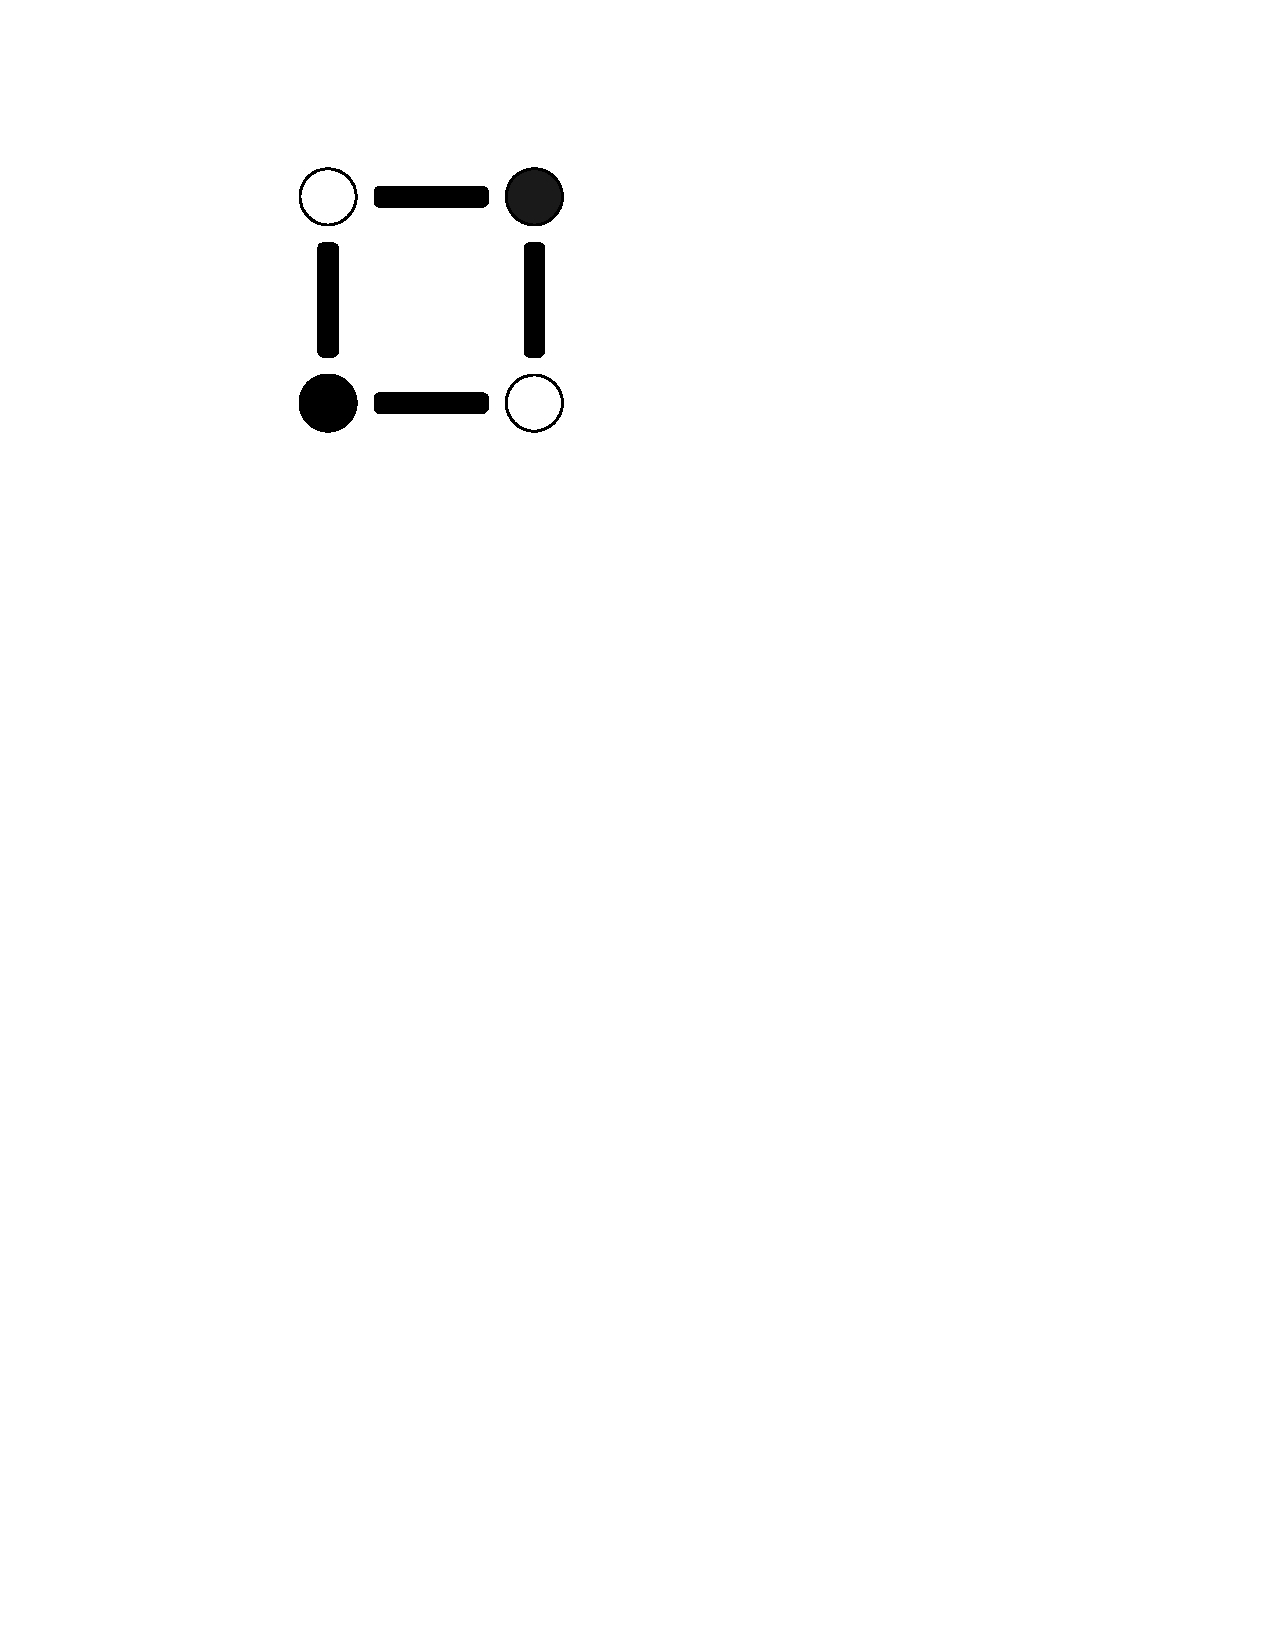
\includegraphics[width=.2\linewidth]{negative.pdf}\label{fig:negative}}
\caption{Positive and negative rectangle contraints. White corresponds to points being added, and black corresponds to the points being subtracted}
\label{fig:rectangles}
\end{figure}

With this, we have simplified our constraints significantly and only lost an $O(1)$ factor to the optimum.

\section{Possible Approaches}

\subsection{Experiments}

We ran experiments to see how the integer linear program compared to the linear program. In particular, we wanted to see whether they were the same, or what the integrality gap was. We wrote a program in python that would generate instances of the points in the plane problem and tried to solve it with the second linear program. We used a python library PuLP which in turn used GLPK (GNU Linear Programming Kit). We were able to run experiments and showed that in fact there are cases for which the second linear program had an integrality gap strictly greater than 1. In most cases, the integrality gap was between 1 and 2, and never surpassed 1.6.

\subsection{Max Flow}

We tried to solve the integer linear program for an optimal solution. This would have solved the points in the plane problem. We wanted to write the integer linear program as an equivalent flow problem. We were unsuccessful at coming up with such a formulation, and we believe that no simple max flow formulations of this exact LP exist. A natural way of rewriting this problem as a flow problem would probably result in a flow problem with integral capacities and costs, given that all coefficients in the constraints in the linear program are integers. However, the Integral Flow Theorem would then guarantee that the optimal solution to this LP would be integral. This cannot be the case, since experimental evidence shows there is an integrality gap strictly greater than 1.

\subsection{The Dual}

The next thing we wanted to do was take the dual to see if we could derive some combinatorial interpretation that could simplify the problem or even find other potential algorithms for the problem.
Representing the linear program as a matrix, the primal linear program looks like:
\[ \min \hspace{.1in} [ \begin{array}{cccc} 1 & 1 & \dots & 1 \end{array} ] \left[\begin{array}{c} b_{11} \\ b_{12} \\ \vdots \\ b_{nn} \end{array} \right]\]
such that
\[ \left[ \begin{array}{c} \vdots \\ \text{ $P$ = positive rectangles } \\ \vdots \\ \text{ $N$ = negative rectangles } \\ \vdots \\ \text{ $I_n'$ = equality } \end{array} \right] 
\left[\begin{array}{c} b_{11} \\ b_{12} \\ \vdots \\ b_{nn} \end{array} \right] 
\begin{array}{c} \\ \leq \\ \\ \\ \leq \\ \\ \\ = \end{array} 
\left[\begin{array}{c} 1 \\\\ 1 \\\\ \vdots \\\\ 1 \end{array} \right] \]

Where $P$ and $N$ are $\dbinom{n}{2}^2 \times n^2$ matrices, since there are that many positive and negative rectangles. $I_n'$ is the some permutation of identity matrix with extra zero columns. Furthermore, we require that all variables are positive. 

We can compute the dual:
\[ \max y^T \left[ \begin{array}{c} 1 \\ 1 \\ \vdots \\ 1 \end{array} \right] \]
such that
\[ \left[ \begin{array}{ccc} \vdots & \vdots & \vdots \\
					  P^T & N^T & I_n \\
					\vdots & \vdots & \vdots \end{array} \right] y
\leq  \left[ \begin{array}{c} 1 \\ 1 \\ \vdots \\ 1 \end{array} \right] \]
Where the first $n$ variables in $y$ can take on any value, and the rest must all be negative. 

This will corresponds to the following:

We will have a variable for each positive rectangle and each negative rectangle, denoted $b_{ij, lk}$ and a variable for each point that was set $a_{xy}$. Then for each point $xy$, if $xy$ is set, then we have the following constraint:
\[ a_{xy} + \sum_{\begin{array}{c}\text{rectangles where}\\\text{$xy$ on corner}\end{array}} b_{ij, lk} - \sum_{\begin{array}{c}\text{rectangles where}\\\text{$xy$ on side}\end{array}} b_{ij,lk} \leq 1 \]
If $xy$ is not set, then the $a_{xy}$ term is not present. We want to maximize
\[ \sum a_{xy} + \sum b_{ij,lk} \]
where $b_{ij,lk} \leq 0$. The $a$'s are unconstrained. We would like to set the values of the rectangles that have points two points on their corners as negative, since then we could raise $a_{xy}$ by the same amount in both corners and thus increase the objective.

\section{An Unbounded Integrality Gap}

We show that the linear programming relaxation will probably not yield an $O(1)$-approximation.

There are known instances of the problem that require $O(n\log n)$ additional points. On one of these instances, if you set all the neighboring points of set points to $0.5$. To see that this solution is feasible, note that every rectangle created from points of value 1 will be satisfied, since the rectangle must contain at least 2 points of value $0.5$. All the rectangles created by one point of value $1$ and one point of value $0.5$ will be satisfied by a point of value $0.5$ adjacent to the point $1$. Finally each rectangle with opposite corners $0.5$ will automatically be satisfied since the sum of the two is already less than or equal to 1. This feasible solution in has an optimum of size $O(n)$; therefore, the integrality gap is $O(\log n)$. 

Figure~\ref{fig:integralitygap} demonstrates the lower bound of the integrality gap. Figure~\ref{fig:optimum} shows the optimum of the integer linear program, where the white circles are the instance of the problem and the green circles are the variables that are set to 1. It is clear from the picture that all constraints are satisfied and that this is the minimum number of points needed. Figure~\ref{fig:lpsolution} gives a $O(n)$ feasible solution to the linear program where the white circles indicate the instance of the problem and the red circles are the points that are assigned to $0.5$. 

\begin{figure}
\centering
\subfigure[Optimal solution to integer linear program]{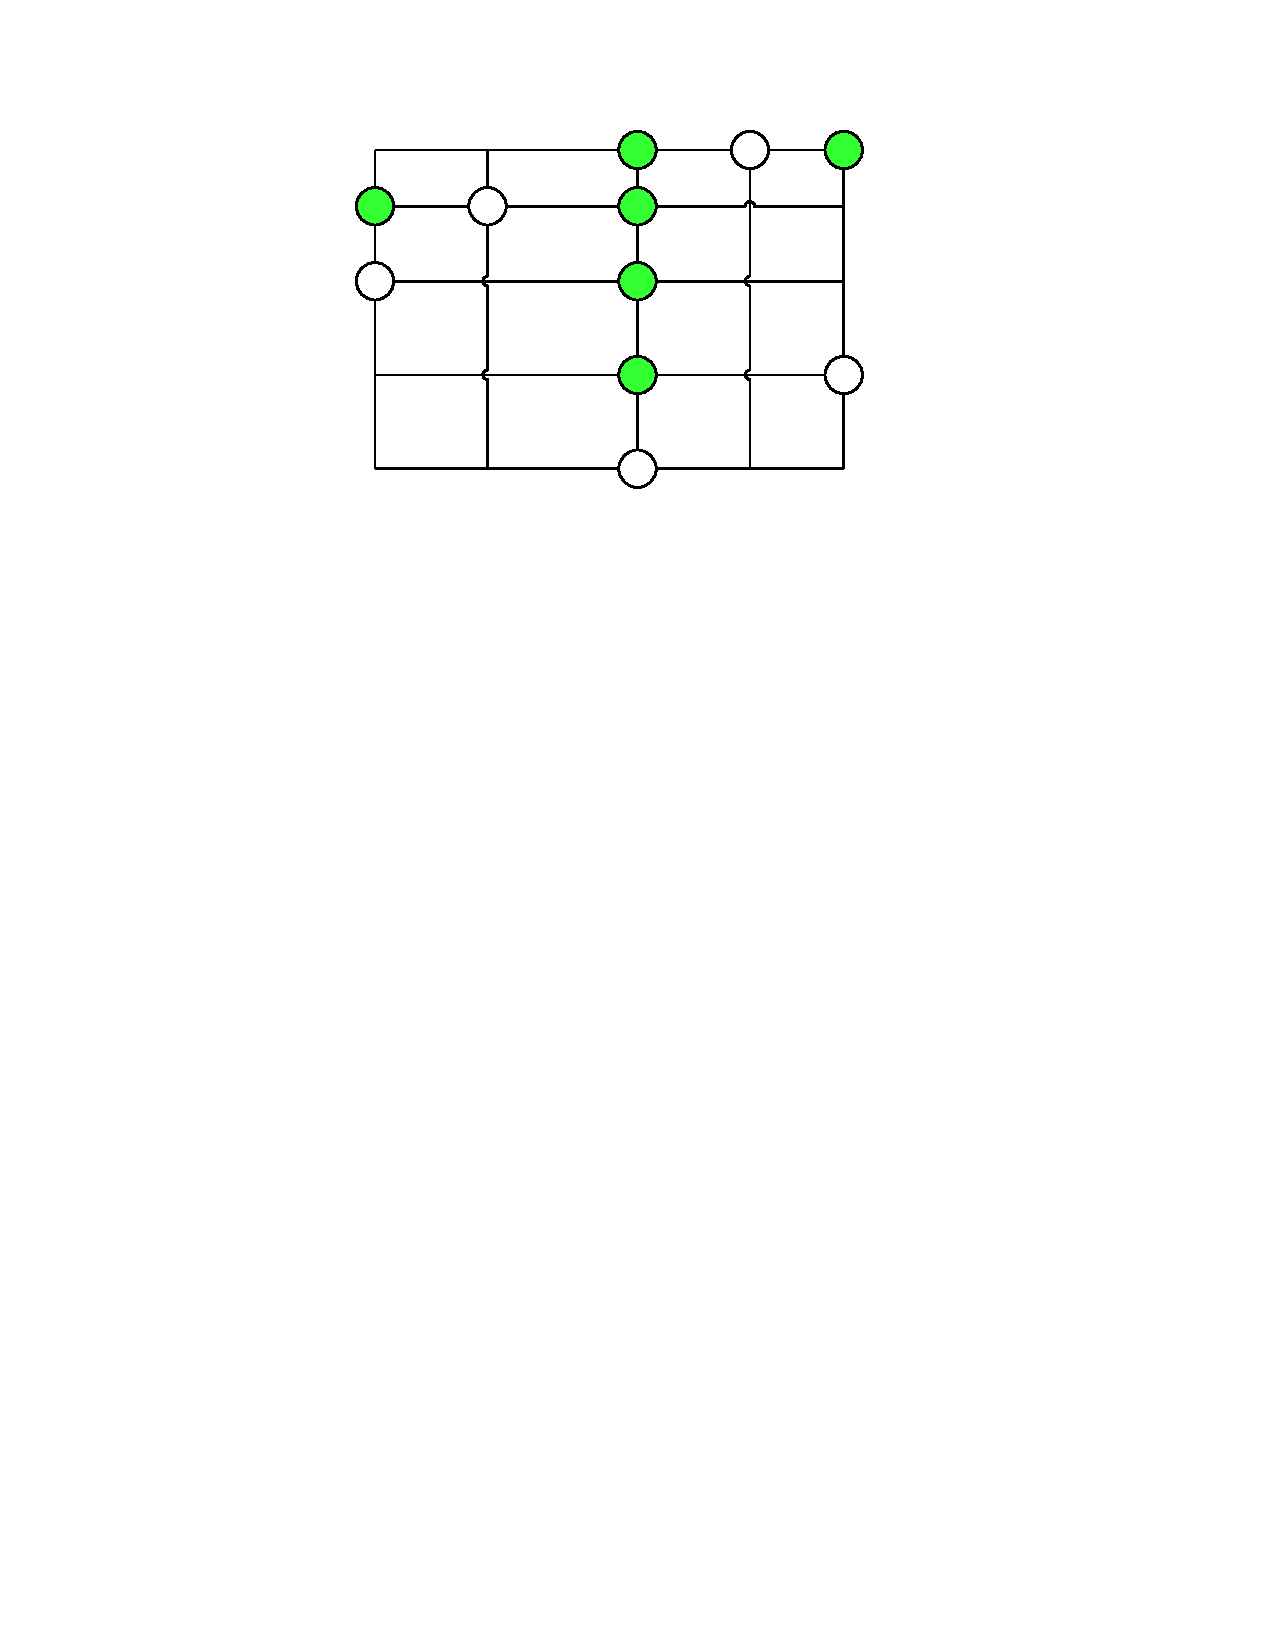
\includegraphics[width=0.4\linewidth]{optimum.pdf}\label{fig:optimum}}
\subfigure[Feasible solution to linear program]{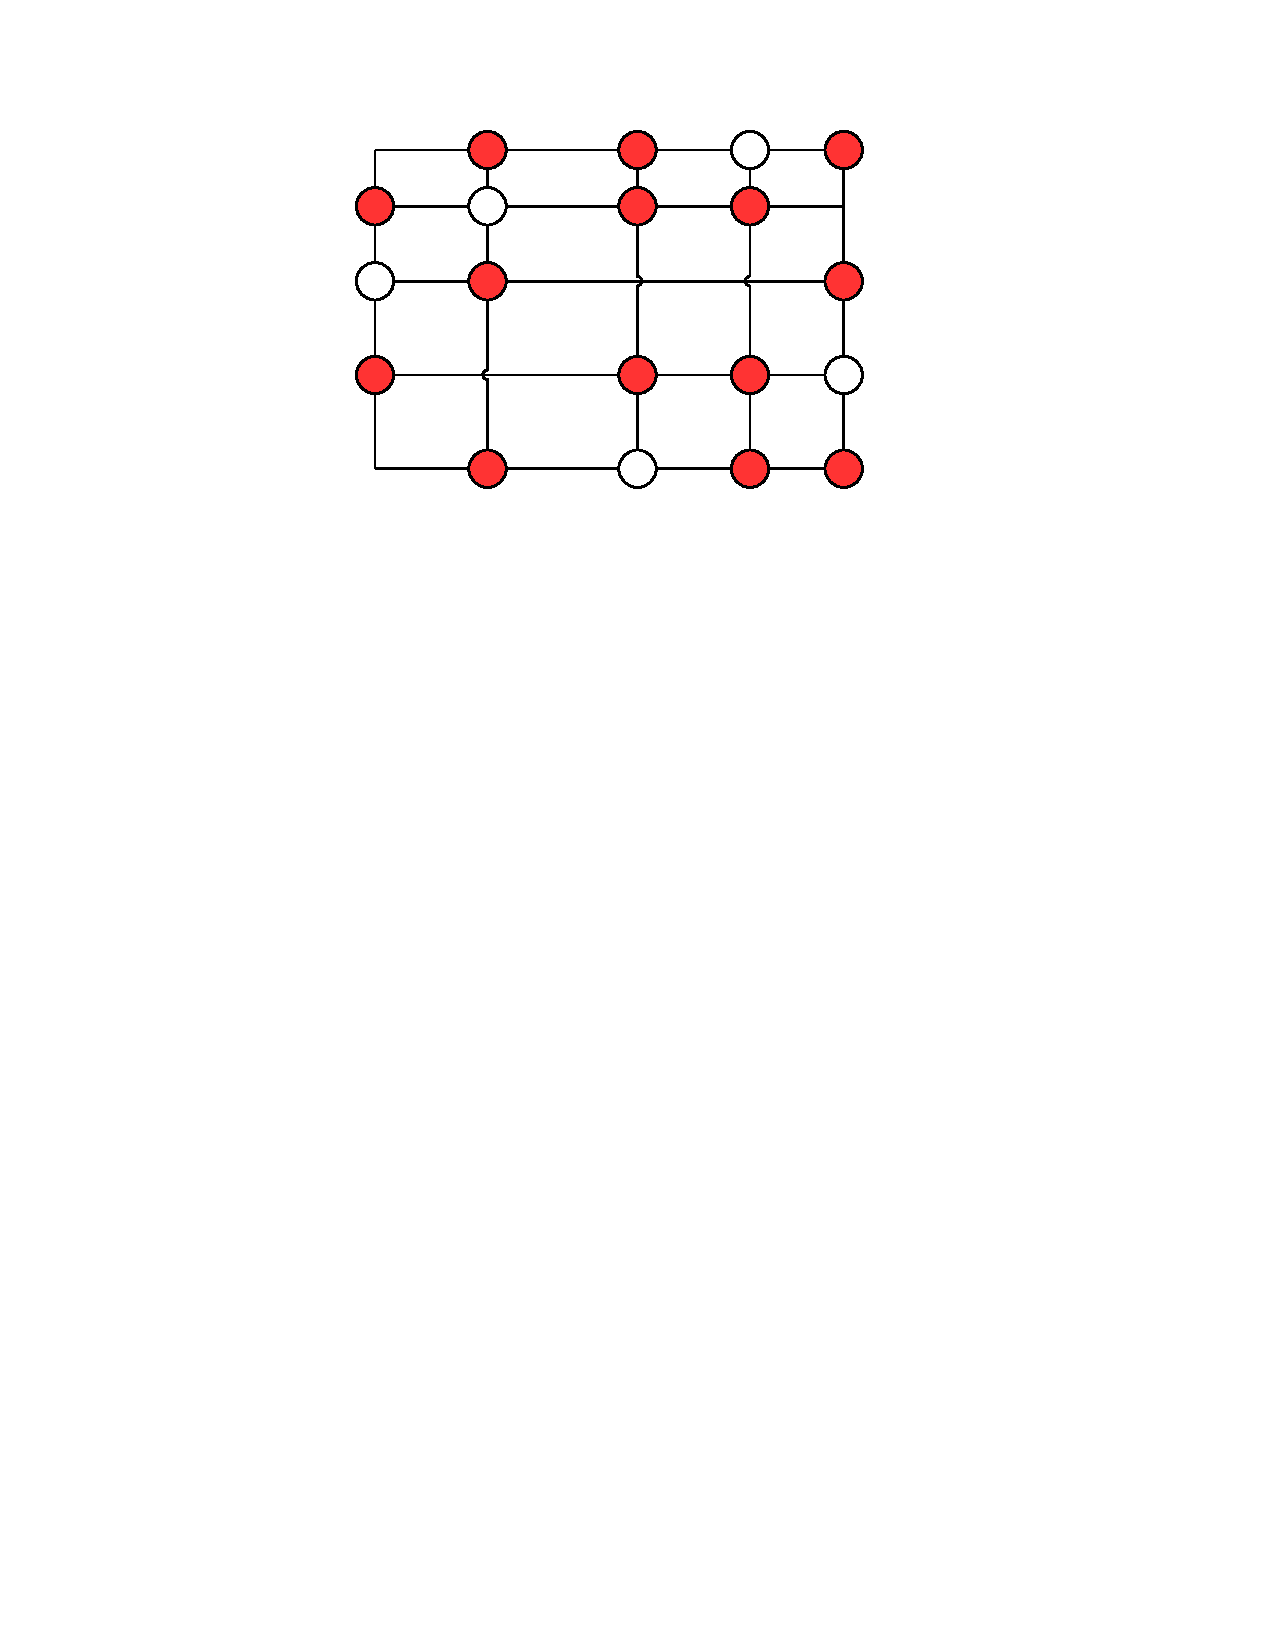
\includegraphics[width=.4\linewidth]{lpsolution.pdf}\label{fig:lpsolution}}
\caption{Integrality gap of linear program}
\label{fig:integralitygap}
\end{figure}

To illustrate how this is a big problem, suppose we had a rounding scheme from the linear programming relaxation. Lets call the rounded solution $R$, $LP$ will be the optimum of the relaxed linear program, and $ILP$ will be the optimum of the integer linear program. What we know is that
\[ LP \leq ILP \leq R \leq O(\log n)LP \]
However, without computing $ILP$, we won't be able to show that $R$ and $ILP$ are close ($O(1)$-factor away). This means that typical rounding scheme proofs won't work. 

\section{Extending the Method}

\section{Conclusions}

\end{document}
